\documentclass[11pt]{article}

\usepackage[margin=1in]{geometry}
\usepackage{tikz}
\usetikzlibrary{arrows.meta, positioning, shapes.geometric, fit}
\usepackage{float}
\usepackage{booktabs}
\usepackage{array}
\usepackage{tabularx}
\usepackage{listings}
\usepackage[table]{xcolor}
\usepackage{hyperref}
\usepackage{enumitem}
\usepackage{caption}
\usepackage{parskip}
\usepackage{titlesec}

% ---- color palette (same as the design report, for a consistent look) ----
\definecolor{navy}{RGB}{21,52,86}
\definecolor{steel}{RGB}{58,110,165}
\definecolor{attackerred}{RGB}{176,42,42}
\definecolor{victimblue}{RGB}{22,86,152}
\definecolor{oklive}{RGB}{27,120,55}
\definecolor{warnamber}{RGB}{191,110,0}
\definecolor{lockred}{RGB}{176,20,20}
\definecolor{panelgray}{RGB}{242,244,247}

\renewcommand{\arraystretch}{1.3}
\renewcommand{\labelitemi}{\textcolor{steel}{\textbullet}}
\renewcommand{\labelenumi}{\textcolor{navy}{\bfseries\theenumi.}}
\raggedbottom

\lstset{
  basicstyle=\ttfamily\small,
  breaklines=true,
  columns=fullflexible,
  frame=single,
  rulecolor=\color{steel!40},
  backgroundcolor=\color{panelgray},
  showstringspaces=false
}

\hypersetup{colorlinks=true, linkcolor=navy, urlcolor=navy, citecolor=navy}

\titleformat{\section}
  {\normalfont\Large\bfseries\color{navy}}{\thesection}{0.6em}{}[{\color{steel}\titlerule[0.8pt]}]
\titleformat{\subsection}
  {\normalfont\large\bfseries\color{navy}}{\thesubsection}{0.6em}{}
\titleformat{\subsubsection}
  {\normalfont\normalsize\bfseries\color{steel}}{\thesubsubsection}{0.6em}{}

% Empty, bordered space reserved for a screenshot or capture image to be
% inserted later. Replace the empty tikzpicture node with
% \includegraphics[width=0.9\textwidth]{path/to/image} when the image is
% ready. The real caption stays outside this box, on the figure itself.
\newcommand{\blankbox}[1]{%
\begin{tikzpicture}
\node[draw=steel, thick, rounded corners, fill=panelgray,
      minimum width=0.9\textwidth, minimum height=#1] {};
\end{tikzpicture}
}

\begin{document}

% ---------------- Cover page ----------------
\begin{titlepage}
\centering
\vspace*{1.2cm}
{\large\bfseries Bangladesh University of Engineering and Technology (BUET)\par}
\vspace{0.25cm}
{\large Department of Computer Science and Engineering\par}

\vspace{2.2cm}
{\color{steel}\rule{0.82\textwidth}{1.4pt}\par}
\vspace{0.7cm}
{\Huge\bfseries\color{navy} Final Report\par}
\vspace{0.5cm}
{\LARGE\bfseries Tool 9: Dictionary Attack\\[2pt] and Known Password Attack\par}
\vspace{0.7cm}
{\color{steel}\rule{0.82\textwidth}{1.4pt}\par}

\vspace{1.8cm}
{\large
\begin{tabular}{ll}
\textbf{Course:} & CSE406: Computer Security Sessional \\
\textbf{Assignment:} & Attack Tool 9 \\
\textbf{Report:} & Final Report and Implementation Demo \\
\end{tabular}
\par}

\vfill

{\large\bfseries\color{navy} Group Members\par}
\vspace{0.4cm}
\begin{tabular}{lll}
\toprule
\rowcolor{navy!12}
\textbf{Member} & \textbf{Student ID} & \textbf{Responsibility} \\
\midrule
Arnob Biswas & 2105015 & Webapp + defense mechanism \\[1.2ex]
Zaki Rehnoom Unmona & 2105016 & Attacker tools + report diagrams \\
\bottomrule
\end{tabular}

\vspace{1.6cm}
{\large \today\par}
\vspace{1cm}
\end{titlepage}

% ---------------- Table of contents ----------------
\pagenumbering{roman}
\tableofcontents
\newpage
\pagenumbering{arabic}
\setcounter{page}{1}

% ==================================================
\section{Overview of the Project}
\label{sec:overview}

We built and demonstrated two related password guessing attacks against a
signup and login webapp that we wrote ourselves, along with a working
defense against both.

\begin{itemize}[leftmargin=*]
  \item \textbf{Dictionary attack.} We target one specific account and try a
    long, ordered list of candidate passwords against it, one at a time,
    until the server accepts one or the list runs out. This works because
    many people choose passwords that show up in common wordlists.
  \item \textbf{Known password attack} (password spraying, or credential
    reuse). Instead of guessing many passwords against one account, we start
    from a small set of known passwords, such as defaults or passwords
    leaked in earlier breaches, and try each one against a wide list of
    accounts. This exploits password reuse and default credentials rather
    than weak individual passwords.
\end{itemize}

The target is a webapp we built from scratch rather than an existing
service, a small signup and login application written in Flask with a
SQLite database. The victim action is a normal user signing up and logging
in through a browser. The attacker action is the two attacks above, driven
by HTTP client code we wrote ourselves, not an existing brute forcing tool.
Alongside the attacks, we built a defense mechanism, account lockout
combined with slow password hashing, so that this report can show the
attacks succeeding and then being stopped once the defense is switched on.

% ==================================================
\section{Network Topology, Components, and Timing Diagrams}
\label{sec:topology}

\subsection{Topology}

We ran the attack on two ordinary devices connected to the same local
network, with no virtual machines involved. The victim device runs the
webapp and is reachable at \texttt{192.168.68.107} on port 5000. The
attacker device sits on the same network and talks to the victim over
plain HTTP. A browser on the same network is used for the legitimate
signup and login action.

\begin{figure}[H]
\centering
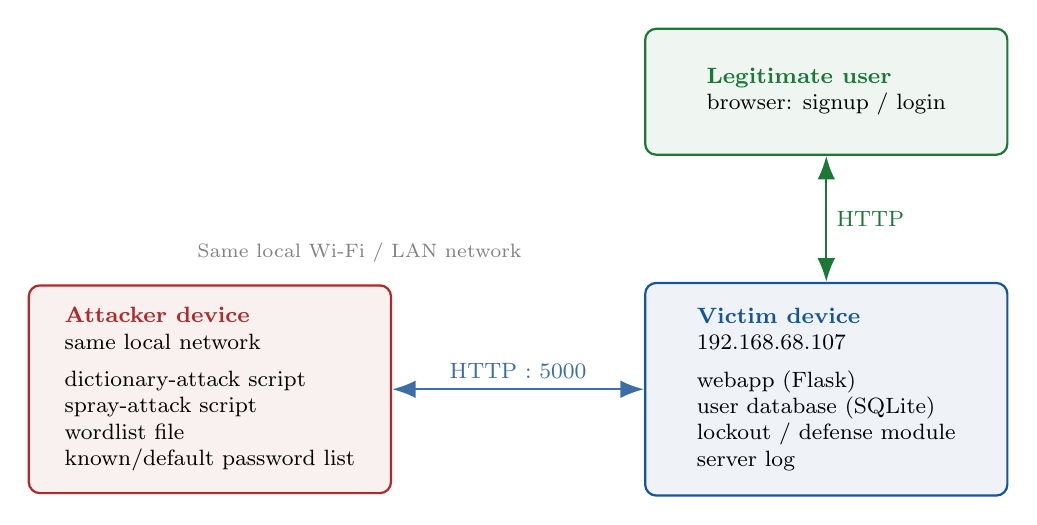
\begin{tikzpicture}[
  attackerbox/.style={draw=attackerred, thick, fill=attackerred!7, rectangle,
    rounded corners, align=left, minimum width=4.6cm, minimum height=2.5cm,
    font=\footnotesize, inner sep=8pt},
  victimbox/.style={draw=victimblue, thick, fill=victimblue!7, rectangle,
    rounded corners, align=left, minimum width=4.6cm, minimum height=2.7cm,
    font=\footnotesize, inner sep=8pt},
  userbox/.style={draw=oklive, thick, fill=oklive!7, rectangle,
    rounded corners, align=left, minimum width=4.6cm, minimum height=1.6cm,
    font=\footnotesize, inner sep=8pt},
  node distance=2.2cm
]
\node[attackerbox] (attacker)
  {\textbf{\color{attackerred}Attacker device} \\ same local network \\[4pt]
   dictionary-attack script \\ spray-attack script \\
   wordlist file \\ known/default password list};

\node[victimbox, right=3.2cm of attacker] (victim)
  {\textbf{\color{victimblue}Victim device} \\ 192.168.68.107 \\[4pt]
   webapp (Flask) \\ user database (SQLite) \\
   lockout / defense module \\ server log};

\node[userbox, above=1.6cm of victim, minimum height=1.6cm] (user)
  {\textbf{\color{oklive}Legitimate user} \\ browser: signup / login};

\draw[{Latex[length=3mm]}-{Latex[length=3mm]}, thick, steel]
  (attacker) -- node[above, font=\footnotesize]{HTTP : 5000} (victim);
\draw[{Latex[length=3mm]}-{Latex[length=3mm]}, thick, oklive]
  (user) -- node[right, font=\footnotesize]{HTTP} (victim);

\node[font=\scriptsize, align=center, text=gray, above=0.15cm of attacker, xshift=1.9cm]
  {Same local Wi-Fi / LAN network};
\end{tikzpicture}
\caption{Attack topology: two devices on the same local network, plus a
legitimate browser client on the same network exercising the webapp. No
virtual machines are used.}
\end{figure}

\subsection{Components}

\begin{table}[H]
\centering
\begin{tabularx}{\textwidth}{@{} l X @{}}
\toprule
\rowcolor{navy!12}
\textbf{Component} & \textbf{Role} \\
\midrule
Victim webapp (Flask) & Serves signup, login, and dashboard pages, the attack target \\
User database (SQLite) & Stores usernames, salts, and password hashes \\
Defense module & Tracks failed login attempts per account and enforces temporary lockout, also selects the slow-hash mode \\
Dictionary-attack script & Attacker tool: many candidate passwords against one account \\
Spray-attack script & Attacker tool: a few known passwords against many accounts \\
Wordlist / known-password list & Input data for the two attacker scripts \\
Server / attacker logs & Record every login attempt and outcome \\
\bottomrule
\end{tabularx}
\caption{System components and their roles.}
\end{table}

\newpage
\subsection{Timing Diagrams}

The diagrams below describe the protocol our webapp implements and the
attack strategies we ran against it. Request arrows (client to server) are
shown in \textcolor{steel}{steel blue}. Responses are colored by outcome:
\textcolor{oklive}{green for success}, \textcolor{warnamber!90!black}{amber
for a failed attempt}, and \textcolor{lockred}{red for a lockout}.

\subsubsection{Normal (legitimate) signup and login: browser flow}

\begin{figure}[H]
\centering
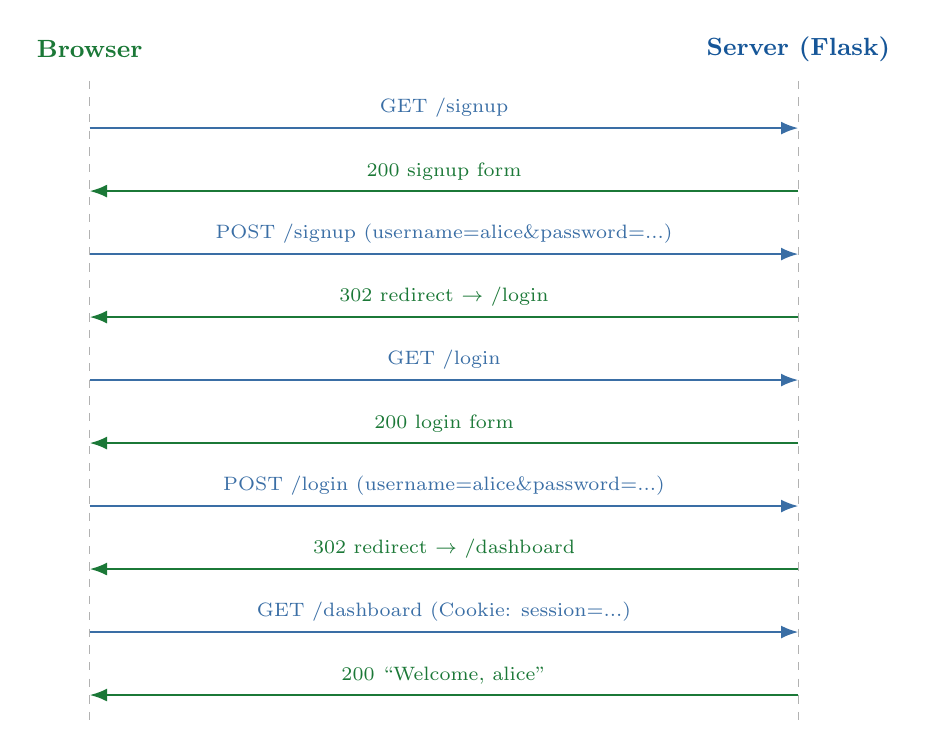
\begin{tikzpicture}[
  reqmsg/.style={-{Latex[length=2.2mm]}, thick, steel},
  okmsg/.style={-{Latex[length=2.2mm]}, thick, oklive},
  lbl/.style={font=\scriptsize, midway, above}
]
\node[font=\bfseries\small, text=oklive] at (0,0.4) {Browser};
\node[font=\bfseries\small, text=victimblue] at (9,0.4) {Server (Flask)};
\draw[dashed, gray!60] (0,0) -- (0,-8.2);
\draw[dashed, gray!60] (9,0) -- (9,-8.2);

\draw[reqmsg] (0,-0.6)  -- (9,-0.6)  node[lbl]{GET /signup};
\draw[okmsg]  (9,-1.4)  -- (0,-1.4)  node[lbl]{200 signup form};
\draw[reqmsg] (0,-2.2)  -- (9,-2.2)  node[lbl]{POST /signup (username=alice\&password=...)};
\draw[okmsg]  (9,-3.0)  -- (0,-3.0)  node[lbl]{302 redirect $\rightarrow$ /login};
\draw[reqmsg] (0,-3.8)  -- (9,-3.8)  node[lbl]{GET /login};
\draw[okmsg]  (9,-4.6)  -- (0,-4.6)  node[lbl]{200 login form};
\draw[reqmsg] (0,-5.4)  -- (9,-5.4)  node[lbl]{POST /login (username=alice\&password=...)};
\draw[okmsg]  (9,-6.2)  -- (0,-6.2)  node[lbl]{302 redirect $\rightarrow$ /dashboard};
\draw[reqmsg] (0,-7.0)  -- (9,-7.0)  node[lbl]{GET /dashboard (Cookie: session=...)};
\draw[okmsg]  (9,-7.8)  -- (0,-7.8)  node[lbl]{200 ``Welcome, alice''};
\end{tikzpicture}
\caption{Normal protocol timing: one legitimate signup followed by one
login.}
\end{figure}

\subsubsection{Dictionary attack: repeated exchange, one account}

\begin{figure}[H]
\centering
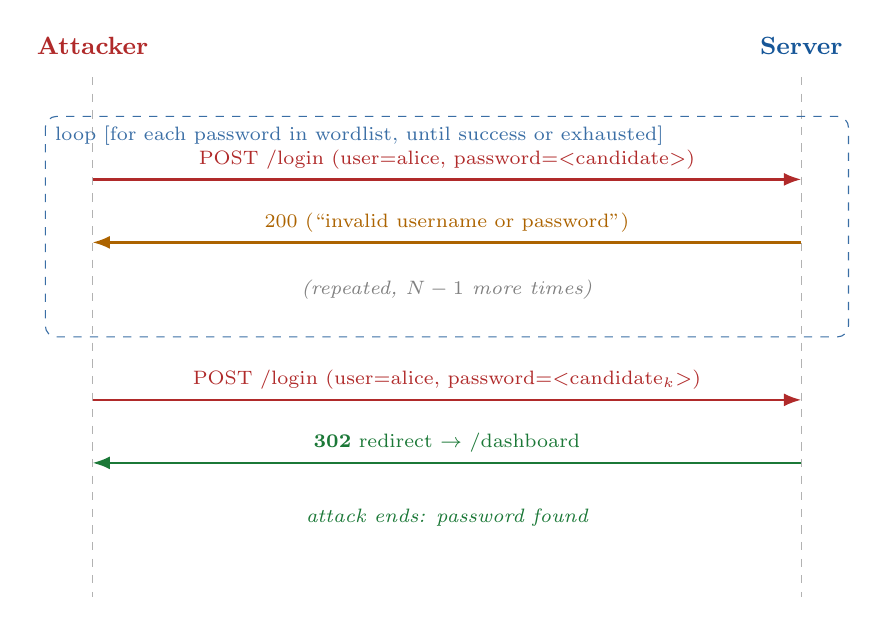
\begin{tikzpicture}[
  reqmsg/.style={-{Latex[length=2.2mm]}, thick, attackerred},
  failmsg/.style={-{Latex[length=2.2mm]}, thick, warnamber!90!black},
  okmsg/.style={-{Latex[length=2.2mm]}, thick, oklive},
  lbl/.style={font=\scriptsize, midway, above}
]
\node[font=\bfseries\small, text=attackerred] at (0,0.4) {Attacker};
\node[font=\bfseries\small, text=victimblue] at (9,0.4) {Server};
\draw[dashed, gray!60] (0,0) -- (0,-6.6);
\draw[dashed, gray!60] (9,0) -- (9,-6.6);

\draw[dashed, steel, rounded corners] (-0.6,-0.5) rectangle (9.6,-3.3);
\node[font=\scriptsize, text=steel, anchor=north west] at (-0.6,-0.5)
  {loop~[for each password in wordlist, until success or exhausted]};

\draw[reqmsg]  (0,-1.3) -- (9,-1.3) node[lbl]{POST /login (user=alice, password=\textless candidate\textgreater)};
\draw[failmsg] (9,-2.1) -- (0,-2.1) node[lbl]{200 (``invalid username or password'')};
\node[font=\scriptsize\itshape, text=gray] at (4.5,-2.7) {(repeated, $N-1$ more times)};

\draw[reqmsg] (0,-4.1) -- (9,-4.1) node[lbl]{POST /login (user=alice, password=\textless candidate$_k$\textgreater)};
\draw[okmsg]  (9,-4.9) -- (0,-4.9) node[lbl]{\textbf{302} redirect $\rightarrow$ /dashboard};
\node[font=\scriptsize\itshape, text=oklive] at (4.5,-5.6) {attack ends: password found};
\end{tikzpicture}
\caption{Dictionary attack: many candidate passwords tried in sequence
against a single account.}
\end{figure}

\subsubsection{Known-password (spray) attack: repeated exchange, many accounts}

\begin{figure}[H]
\centering
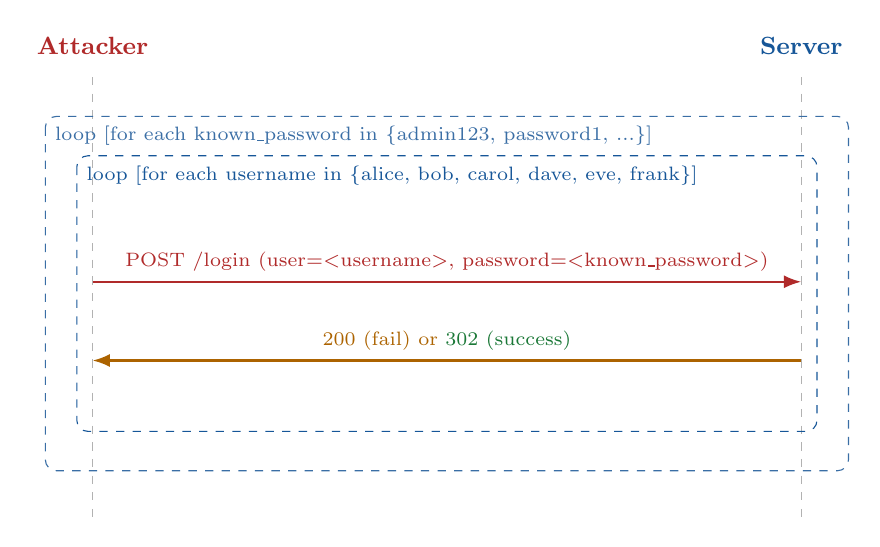
\begin{tikzpicture}[
  reqmsg/.style={-{Latex[length=2.2mm]}, thick, attackerred},
  mixmsg/.style={-{Latex[length=2.2mm]}, thick, warnamber!90!black},
  lbl/.style={font=\scriptsize, midway, above}
]
\node[font=\bfseries\small, text=attackerred] at (0,0.4) {Attacker};
\node[font=\bfseries\small, text=victimblue] at (9,0.4) {Server};
\draw[dashed, gray!60] (0,0) -- (0,-5.6);
\draw[dashed, gray!60] (9,0) -- (9,-5.6);

\draw[dashed, steel, rounded corners] (-0.6,-0.5) rectangle (9.6,-5.0);
\node[font=\scriptsize, text=steel, anchor=north west] at (-0.6,-0.5)
  {loop~[for each known\_password in \{admin123, password1, ...\}]};

\draw[dashed, victimblue, rounded corners] (-0.2,-1.0) rectangle (9.2,-4.5);
\node[font=\scriptsize, text=victimblue, anchor=north west] at (-0.2,-1.0)
  {loop~[for each username in \{alice, bob, carol, dave, eve, frank\}]};

\draw[reqmsg] (0,-2.6) -- (9,-2.6) node[lbl]{POST /login (user=\textless username\textgreater, password=\textless known\_password\textgreater)};
\draw[mixmsg] (9,-3.6) -- (0,-3.6) node[lbl]{\textcolor{warnamber!90!black}{200 (fail)} or \textcolor{oklive}{302 (success)}};
\end{tikzpicture}
\caption{Known-password / spray attack: few known passwords tried across
many accounts.}
\end{figure}

\subsubsection{With the lockout defense active}

\begin{figure}[H]
\centering
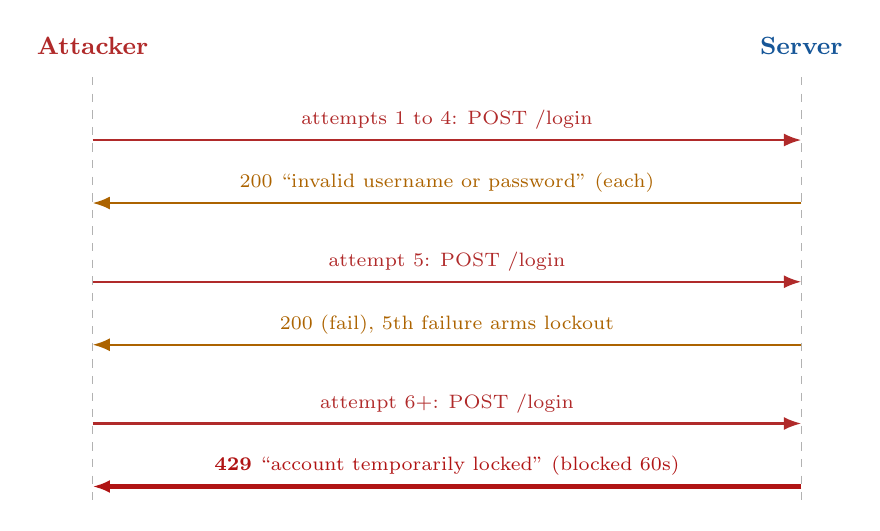
\begin{tikzpicture}[
  reqmsg/.style={-{Latex[length=2.2mm]}, thick, attackerred},
  failmsg/.style={-{Latex[length=2.2mm]}, thick, warnamber!90!black},
  lockmsg/.style={-{Latex[length=2.2mm]}, ultra thick, lockred},
  lbl/.style={font=\scriptsize, midway, above}
]
\node[font=\bfseries\small, text=attackerred] at (0,0.4) {Attacker};
\node[font=\bfseries\small, text=victimblue] at (9,0.4) {Server};
\draw[dashed, gray!60] (0,0) -- (0,-5.4);
\draw[dashed, gray!60] (9,0) -- (9,-5.4);

\draw[reqmsg]  (0,-0.8) -- (9,-0.8) node[lbl]{attempts 1 to 4: POST /login};
\draw[failmsg] (9,-1.6) -- (0,-1.6) node[lbl]{200 ``invalid username or password'' (each)};

\draw[reqmsg]  (0,-2.6) -- (9,-2.6) node[lbl]{attempt 5: POST /login};
\draw[failmsg] (9,-3.4) -- (0,-3.4) node[lbl]{200 (fail), 5th failure arms lockout};

\draw[reqmsg]  (0,-4.4) -- (9,-4.4) node[lbl]{attempt 6+: POST /login};
\draw[lockmsg] (9,-5.2) -- (0,-5.2) node[lbl]{\textbf{429} ``account temporarily locked'' (blocked 60s)};
\end{tikzpicture}
\caption{Lockout defense: the dictionary and spray attacks are blocked
after 5 failed attempts within a 30-second window.}
\end{figure}

% ==================================================
\section{Packet and Frame Structure}
\label{sec:packet}

No raw Ethernet or IP crafting is needed for this attack, since the exploit
sits entirely at the application layer, carried over an ordinary TCP
connection. The transport is standard TCP carrying HTTP/1.1, using Flask's
built-in development server. What we designed from scratch is the
application behaviour and the payload the HTTP request carries, and how
the server interprets it, not an existing authentication protocol
implementation.

\subsection{Request (attacker or browser to server), one per login attempt}

\begin{lstlisting}
POST /login HTTP/1.1
Host: 192.168.68.107:5000
Content-Type: application/x-www-form-urlencoded
Content-Length: 33

username=alice&password=sunshine
\end{lstlisting}

\subsection{Responses, by outcome}

\begin{table}[H]
\centering
\begin{tabularx}{\textwidth}{@{} l l X @{}}
\toprule
\rowcolor{navy!12}
\textbf{Outcome} & \textbf{Status} & \textbf{Notable headers / body} \\
\midrule
\textcolor{oklive}{\textbf{Success}} & \texttt{302 FOUND} & \texttt{Location: /dashboard}, \texttt{Set-Cookie: session=...} \\
\textcolor{warnamber!90!black}{\textbf{Failure}} & \texttt{200 OK} & login page HTML containing ``invalid username or password'' \\
\textcolor{lockred}{\textbf{Locked}} (defense on) & \texttt{429 TOO MANY REQUESTS} & login page HTML containing ``account temporarily locked'' \\
\bottomrule
\end{tabularx}
\caption{HTTP response codes and bodies for each login outcome.}
\end{table}

\subsection{Design Notes}

\begin{itemize}[leftmargin=*]
  \item Each attempt opens its own TCP connection, since the attacker
    scripts issue one HTTP request per attempt with no session reuse: a
    full three-way handshake, the HTTP request and response, then a
    FIN/ACK teardown, for every attempt. We captured this on the wire
    between the two devices with Wireshark, shown below.
  \item Whether the username does not exist or the password is simply
    wrong, the response to a failed login is the same generic message,
    ``invalid username or password'', so the app never leaks whether an
    account exists.
  \item Passwords are sent as cleartext form data over plain HTTP, with no
    TLS. This is a deliberate simplification, consistent with the
    assignment's other plaintext-protocol attacks, and it is worth noting
    as a limitation compared to a production deployment, which would use
    HTTPS.
\end{itemize}

% ==================================================
\section{Test Environment}
\label{sec:environment}

The results in this report come from an actual two-device setup on the same
local network, not from virtual machines and not from a single machine over
loopback.

\begin{itemize}[leftmargin=*]
  \item \textbf{Victim device.} Runs the Flask webapp bound to all
    interfaces, reachable at \texttt{http://192.168.68.107:5000} from the
    rest of the network. Started undefended with \texttt{python seed.py}
    followed by \texttt{python app.py}, which hashes passwords with a
    single fast salted SHA-256 and enforces no lockout. Started defended
    with a fresh \texttt{app.db}, \texttt{python seed.py --defense}, and
    \texttt{DEFENSE=1 python app.py}, which hashes with salted
    PBKDF2-HMAC-SHA256 at 200{,}000 iterations and turns the lockout
    tracker on.
  \item \textbf{Attacker device.} On the same local network as the victim,
    pointed at \texttt{http://192.168.68.107:5000}. Runs
    \texttt{attacker\_dict.py} against the account \texttt{alice} using
    \texttt{wordlist.txt} (1000 candidate passwords), and
    \texttt{attacker\_spray.py} against the six accounts in
    \texttt{targets.txt} using the 33 passwords in
    \texttt{known\_passwords.txt}.
\end{itemize}

\begin{figure}[H]
\centering
\blankbox{3.2cm}
\caption{Network interface output from the victim device and the attacker
device, showing both are on the 192.168.68.0/24 network.}
\end{figure}

% ==================================================
\section{Steps of the Attacks}
\label{sec:steps}

\subsection{Victim action: a normal signup and login}

Before running either attack, we exercised the webapp the way a normal user
would, to confirm the signup and login flow works on its own.

\begin{enumerate}[leftmargin=*]
  \item Open \texttt{http://192.168.68.107:5000/signup} in a browser and
    create a new account.
  \item Log in with the same account at \texttt{/login}.
  \item Land on \texttt{/dashboard}, which only shows once the login
    succeeds.
\end{enumerate}

\begin{figure}[H]
\centering
\blankbox{5cm}
\caption{Browser screenshots of the signup page, the login page, and the
dashboard after a normal login.}
\end{figure}

\subsection{Dictionary attack, step by step}

\begin{enumerate}[leftmargin=*]
  \item Start the victim webapp, undefended or defended.
  \item From the attacker device, run \\
    \texttt{python attacker\_dict.py --url http://192.168.68.107:5000 --user alice --wordlist wordlist.txt}
  \item The script sends one \texttt{POST /login} request per candidate
    password in the wordlist, in order, and reads the HTTP status code
    back.
  \item It stops as soon as it sees \texttt{302} (password found),
    \texttt{429} (locked out), or the wordlist runs out.
\end{enumerate}

\subsection{Known password (spray) attack, step by step}

\begin{enumerate}[leftmargin=*]
  \item Start the victim webapp, undefended or defended.
  \item From the attacker device, run \\
    \texttt{python attacker\_spray.py --url http://192.168.68.107:5000 --userlist targets.txt --passwords known\_passwords.txt}
  \item The script tries one known password against every account in the
    target list before moving on to the next known password.
  \item It records every attempt and every account where a \texttt{302}
    came back.
\end{enumerate}

\begin{figure}[H]
\centering
\blankbox{5cm}
\caption{Side by side terminal screenshots: the attacker device running
each script, and the victim device's server log scrolling at the same
time.}
\end{figure}

% ==================================================
\section{Observations}
\label{sec:observations}

This section is the core of the report. For each attack, in each mode, we
describe what we expected from the Design Report, what actually happened
according to our own logs from the two-device run, and, where the two do
not match exactly, why we think that is. All log excerpts below are copied
directly from \texttt{src/logs/attacker\_dict.log},
\texttt{src/logs/attacker\_spray.log}, and \texttt{src/logs/server.log},
with only the surrounding noise trimmed.

\subsection{Dictionary attack, undefended}

\textbf{What we expected.} Since \texttt{alice}'s password \texttt{sunshine}
is inside \texttt{wordlist.txt}, we expected the attack to find it well
before the list ran out, and to do so quickly, since every hash check is a
single fast SHA-256.

\textbf{What we observed.} The attack found the password on attempt 49 out
of 1000, in about 2 seconds of wall clock time, at roughly 35 to 50
milliseconds per attempt.

\begin{lstlisting}
[  1.684s] attempt=41 user=alice password='asdfgh' -> HTTP 200
[  1.732s] attempt=42 user=alice password='hunter' -> HTTP 200
[  1.755s] attempt=43 user=alice password='buster' -> HTTP 200
[  1.794s] attempt=44 user=alice password='soccer' -> HTTP 200
[  1.840s] attempt=45 user=alice password='harley' -> HTTP 200
[  1.863s] attempt=46 user=alice password='batman' -> HTTP 200
[  1.905s] attempt=47 user=alice password='andrew' -> HTTP 200
[  1.927s] attempt=48 user=alice password='tigger' -> HTTP 200
[  1.963s] attempt=49 user=alice password='sunshine' -> HTTP 302
CRACKED user=alice password=sunshine attempts=49 time=1.96s
\end{lstlisting}

\textbf{Match or not.} This matches what we expected. The password was
found inside the wordlist, near the top few percent of it, and the attack
needed only a couple of seconds of real network traffic to succeed. We
reproduced this same result, attempt 49, across several separate runs,
which tells us the behaviour is stable and not a one time fluke.

\begin{figure}[H]
\centering
\blankbox{4.5cm}
\caption{Wireshark capture of the dictionary attack traffic between the
attacker and victim devices, Follow HTTP Stream view of one attempt.}
\end{figure}

\subsection{Dictionary attack, defended}

\textbf{What we expected.} With the lockout set to 5 failed attempts inside
30 seconds, an attacker who does not already know the password should get
locked out after the 5th failure, well before reaching attempt 49. We also
expected each attempt to take noticeably longer because of the slower
PBKDF2 hash.

\textbf{What we observed.} The account was locked out on attempt 6, before
the correct password was ever tried.

\begin{lstlisting}
[  0.131s] attempt=1 user=alice password='123456' -> HTTP 200
[  0.252s] attempt=2 user=alice password='password' -> HTTP 200
[  0.352s] attempt=3 user=alice password='12345678' -> HTTP 200
[  0.487s] attempt=4 user=alice password='qwerty' -> HTTP 200
[  0.587s] attempt=5 user=alice password='123456789' -> HTTP 200
[  0.635s] attempt=6 user=alice password='12345' -> HTTP 429
LOCKED_OUT user=alice attempts=6 time=0.63s
\end{lstlisting}

\textbf{Match or not.} This matches the design closely. The attack is cut
short well before it can reach \texttt{sunshine} at position 49, so a
dictionary attack that succeeded in the undefended run is completely
blocked here. On timing, we measured each attempt taking longer, around
100 to 135 milliseconds per attempt here against roughly 35 to 50
milliseconds in the undefended run, so about two to three times slower.
This is a smaller gap than the roughly 200{,}000 times more hashing work
that PBKDF2 at 200{,}000 iterations actually does per check. The reason is
that this measurement is the whole HTTP round trip across the network,
which also includes the Flask development server and Python, not the hash
function alone. The extra hashing cost is real, but here it is an addition
on top of a larger fixed cost. A cleaner way to see the full effect would
be timing the hash function directly rather than the full request.

\subsection{Known password attack, undefended}

\textbf{What we expected.} Since \texttt{eve} and \texttt{frank} share the
password \texttt{admin123}, and none of \texttt{alice}, \texttt{bob},
\texttt{carol}, or \texttt{dave} use any password from
\texttt{known\_passwords.txt}, we expected the first pass of the spray
attack to compromise exactly those two accounts and nothing else.

\textbf{What we observed.} Both accounts were compromised on the very first
known password tried, and no other account was ever compromised across the
full run of 33 known passwords against 6 accounts.

\begin{lstlisting}
[  0.042s] user=alice password='admin123' -> HTTP 200
[  0.088s] user=bob password='admin123' -> HTTP 200
[  0.134s] user=carol password='admin123' -> HTTP 200
[  0.158s] user=dave password='admin123' -> HTTP 200
[  0.182s] user=eve password='admin123' -> HTTP 302
CRACKED user=eve password=admin123
[  0.206s] user=frank password='admin123' -> HTTP 302
CRACKED user=frank password=admin123
\end{lstlisting}

\textbf{Match or not.} This matches exactly. The attack needed only one
guess per compromised account, which is the whole point of a known
password attack: it does not need a large wordlist, it needs the right
guess to be shared across accounts.

\subsection{Known password attack, defended}

\textbf{What we expected.} Based on the Design Report, we expected the
lockout to throttle this attack per account, the same way it throttles the
dictionary attack.

\textbf{What we observed.} \texttt{eve} and \texttt{frank} were compromised
immediately, exactly as in the undefended run. The lockout only affected
the accounts that were never going to be compromised anyway.

\begin{lstlisting}
[  0.047s] user=alice password='admin123' -> HTTP 429
[  0.196s] user=bob password='admin123' -> HTTP 200
[  0.321s] user=carol password='admin123' -> HTTP 200
[  0.468s] user=dave password='admin123' -> HTTP 200
[  0.616s] user=eve password='admin123' -> HTTP 302
CRACKED user=eve password=admin123
[  0.716s] user=frank password='admin123' -> HTTP 302
CRACKED user=frank password=admin123
[  0.739s] user=alice password='password1' -> HTTP 429
        ...
[  3.420s] user=alice password='Welcome1' -> HTTP 429
[  3.467s] user=bob password='Welcome1' -> HTTP 429
[  3.513s] user=carol password='Welcome1' -> HTTP 429
[  3.561s] user=dave password='Welcome1' -> HTTP 429
\end{lstlisting}

\textbf{Match or not, and why it differs.} This is the one place where our
actual result does not match what we expected in the Design Report, and it
is worth explaining clearly. The lockout only ever counts a \emph{failed}
attempt. For \texttt{eve} and \texttt{frank}, the very first password we
try against them is already the correct one, so the request that
compromises them is a success, not a failure, and it happens before the
lockout counter has any failures to count. The lockout only has time to
build up against \texttt{bob}, \texttt{carol}, and \texttt{dave}, who fail
every single password we try, which is why they end up locked out after
enough wrong guesses, even though they were never actually vulnerable to
this attack in the first place. \texttt{alice} shows as locked from the
very first line here because a dictionary attack against her had already
used up her five failures moments earlier in the same test session, so her
lockout was still active.

The lesson we take from this is that account lockout, on its own, is a good
defense against a dictionary attack, where the attacker has to fail many
times before finding the right password, but it does very little against a
known password attack aimed at an account that actually reuses a guessed
password, because that account is compromised on the first try, before any
failure count can matter. Stopping that case would need a different kind
of defense, for example blocking known weak or breached passwords at
signup time so that no account can ever have \texttt{admin123} as its
password, or rate limiting logins per source IP address rather than only
per username, or requiring a second factor for login regardless of how
many failures have happened.

\begin{figure}[H]
\centering
\blankbox{4.5cm}
\caption{Wireshark capture of the spray attack traffic against the
defended server, with the 429 response visible for one of the throttled
accounts.}
\end{figure}

% ==================================================
\section{Assumptions}
\label{sec:assumptions}

Our attacks and our measurements rest on a number of assumptions. We list
them here so the results above are read in the right context.

\begin{itemize}[leftmargin=*]
  \item \textbf{The attacker already knows the target usernames.} Both
    attacker scripts take a username or a list of usernames as input. We do
    not model how an attacker would first learn valid usernames, for
    example from a data breach, from an email naming pattern, or from the
    signup page leaking whether a username is taken.
  \item \textbf{The attacker has direct, unrestricted access to the login
    endpoint.} There is no firewall, web application firewall, CAPTCHA, or
    upstream rate limiter between the attacker and the webapp in our setup.
    A real deployment would likely have at least one of these, which would
    change the numbers in this report.
  \item \textbf{The attacker sends requests back to back with no delay of
    its own.} Our scripts do not deliberately slow themselves down or
    randomize timing to avoid detection. A more careful attacker might
    spread requests out over a longer time to stay under a lockout window,
    which our current lockout defense, with its fixed 30 second window,
    would not fully catch either.
  \item \textbf{The lockout tracker lives in the memory of a single Flask
    process.} If the victim ran multiple app instances behind a load
    balancer, each instance would keep its own separate lockout state, and
    an attacker spread across instances could get more effective guesses
    than our single process test shows.
  \item \textbf{The slow hash defense is aimed at a different threat than
    the one we directly tested.} We tested it through the login endpoint,
    where the bottleneck is dominated by the web request itself, not by the
    hash. Its real target is an attacker who has already stolen the
    password hash table and is guessing offline, with no server and no
    lockout in the way at all. We did not run that offline scenario here,
    since it is outside what the login endpoint alone can demonstrate.
  \item \textbf{Timing numbers reflect the local network conditions at the
    time of testing.} They can vary with Wi-Fi congestion, distance from
    the access point, or a different network entirely.
\end{itemize}

% ==================================================
\section{Defense Mechanism: Design and Assessment}
\label{sec:defense}

We built two defenses into the webapp, both controlled by one
\texttt{DEFENSE} flag so that the exact same attacker scripts can be
pointed at either configuration.

\begin{enumerate}[leftmargin=*]
  \item \textbf{Account lockout.} The server tracks failed login attempts
    per username in memory. After 5 failures within a 30 second window, the
    account is locked for 60 seconds, and every request in that window
    gets back \texttt{429} regardless of the password sent.
  \item \textbf{Slow password hashing.} In defended mode, passwords are
    hashed with salted PBKDF2-HMAC-SHA256 at 200{,}000 iterations instead
    of a single salted SHA-256 hash.
\end{enumerate}

Based on the observations above, we assess the two parts of our defense
separately.

\begin{table}[H]
\centering
\begin{tabularx}{\textwidth}{@{} l X X @{}}
\toprule
\rowcolor{navy!12}
& \textbf{Expected} & \textbf{Actually observed} \\
\midrule
Dictionary attack, defended & Blocked by lockout before reaching the
correct password & Blocked at attempt 6, matches expectation \\
Spray attack, defended & Throttled per account & Still succeeds
immediately on accounts with a shared weak password, only slows down the
accounts that were never actually vulnerable, does not match our original
expectation \\
Cost per login attempt & Higher, on the order of $2 \times 10^5$ more hash
operations & Measurably higher, roughly two to three times slower end to
end, smaller than the theoretical gap because of fixed request overhead \\
\bottomrule
\end{tabularx}
\caption{Expected versus actually observed effect of the lockout and slow
hash defense.}
\end{table}

The lockout works exactly as designed against the dictionary attack, and it
does add real cost to every login attempt as designed, but it does not
fully deliver on what we expected for the spray attack. That gap is not a
bug in our implementation, it is a real limitation of what a per account
failure counter can ever catch. We think this is a useful finding on its
own, since it shows why real systems that care about credential stuffing
usually add more than just a lockout, such as breached password
blocklists, per IP rate limits, or multi factor authentication.

% ==================================================
\section{Conclusion}
\label{sec:conclusion}

We showed that a dictionary attack and a known password attack can both
compromise a realistic signup and login webapp, and that a lockout and
slow hashing defense meaningfully changes that outcome, though not in
exactly the way we first expected. The dictionary attack cracked a weak
password in seconds when undefended and was fully blocked once the lockout
was turned on. The known password attack cracked every account that reused
a guessed default password, in both the undefended and the defended
configuration, which points to a real limitation of a lockout that only
counts failures: it cannot stop an attack whose whole point is to succeed
on the first try.

The webapp, both attacker scripts, and the defense described in this
report are implemented and were tested end to end on two separate devices
over a real local network, using the exact commands and log evidence shown
above.

\end{document}
